\section{Approximation Algorithms}
Supposing we want to solve an NP problem, what we should do? Sacrifice one of three desired features:

\begin{itemize}
    \item{Polynomial time run}
    \item{Solves arbitrary instances of the problem}
    \item{Always returns the optimum}
\end{itemize}

The ρ-approximation algorithms resolves the first 2 problems while return the solution with a factor ρ from the optimum, the challenge is to prove that a solution is close to the optimum without even knowing the optimum.

\begin{itemize}
    \item{Additive Approximation}: What we hope for: $SOL \leq OPT + C$
    \item{Costant Factor Approximation}: The most common: $SOL \leq OPT * C$
    \item{Polynomial Approximation Factor}: $SOL \leq (1+\epsilon)OPT $
\end{itemize}

\subsection{Load Balancing}
We have m identical machines , n $\geq$ m jobs, job j has processing time $t_{j}$, every machine can process at most 1 process at a time, and one process, once started cannot be stopped.\\
Let $S[i]$ be the subset of jobs assigned to the machine i,The load of machine i is L[i] = $\sum j \in S[i] t$, the makespan is the maximum load of every machine $L=max_{i}L_{i}$, our goal is to assign each job to a machine, in order to minimize the makespan.

\begin{figure}[H]
    \centering
    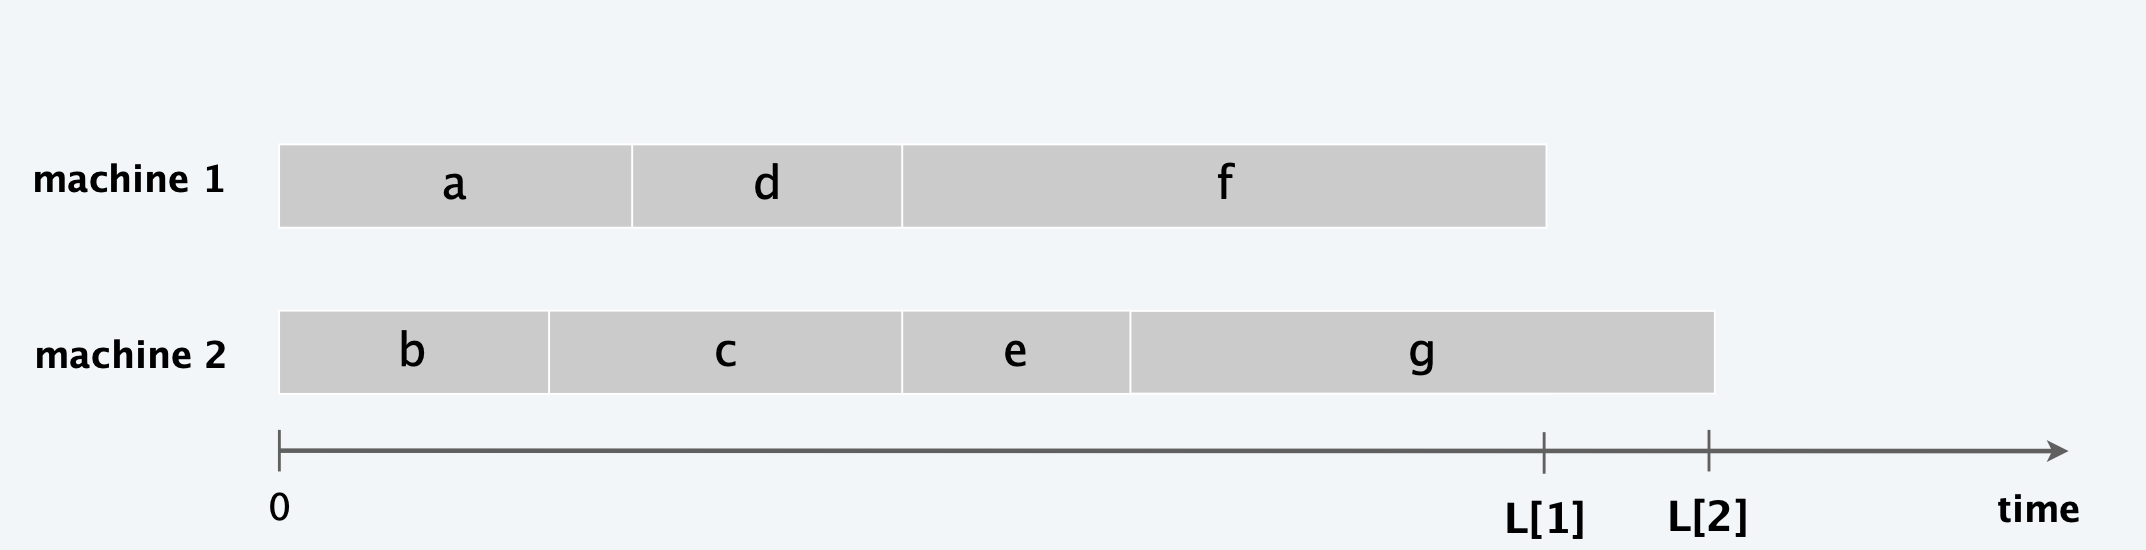
\includegraphics[width=0.6\textwidth ]{loadBalancing}
    \caption{Instance of Load Balancing problem}
\end{figure}

\emph{The list-scheduling algorithm}
Greedy algorithm that does the following: $\forall j \in J$ assign the job to the machine with the smallest amount of load.\\

\begin{claim}
    The optimal makespan is $L^{*} \geq \frac{1}{m} \sum _{k} t_{k}$
\end{claim}\\

\begin{proof}
    The total processing time is $\sum_{k} t_{k}$ , so one of m machines must do at least a 1 / m fraction of total work.
\end{proof}\\

\begin{claim}
    The greedy algorithm is a 2-approximation algorithm.
\end{claim}\\

\begin{proof}
    Consider load L[i] of bottleneck machine i, let j be last job scheduled on machine when this job is assigned. the machine i has the smallest load, hence $L[i]– tj \leq L[k] \; for \; all \; 1 \leq k \leq m$.
\end{proof}\\

Is it possible to make an algorithm that get closer to the optimum? yes.\\
\emph{Longest processing time (LPT)}: Sort n jobs in decreasing order of processing times; then run list scheduling algorithm.\\

\begin{claim}
    LPT rule is a 3/2-approximation algorithm.
\end{claim}\\

\begin{proof}
    Consider load L[i] of bottleneck machine i and let j be last job scheduled on machine i:
    \[ L = L[i] = (L[i] -t_{j}) + t_{j} \leq \frac{3}{2} L^{*}\]
    There exist a more sophisticated analysis of this algorithm that bound the optimum at 4/3.
\end{proof}

\subsection{Center Selection Problem}
We have a set of sites S and an integer k, select a set of k centers C so that maximum distance r(C) from a site to nearest center is minimized.\\\\
Notation:
\begin{itemize}
    \item{dist(x, y) = distance between sites x and y.}
    \item{dist($s_{i}$, C) = min $c \in C$ $dist(s_{i}, c)$ = distance from $s_{i}$ to closest center.}
    \item{r(C) = $max_{i} \; dist(s_{i}, C)$ = smallest covering radius.}
    \item{dist(x, x) = 0 (identity)}
    \item{dist(x, y) = dist(y, x) (simmetry)}
    \item{dist(x, y) $\leq$ dist(x, z) + dist(z, y) (triangle inequality)}

\end{itemize}

\begin{figure}[H]
    \centering
    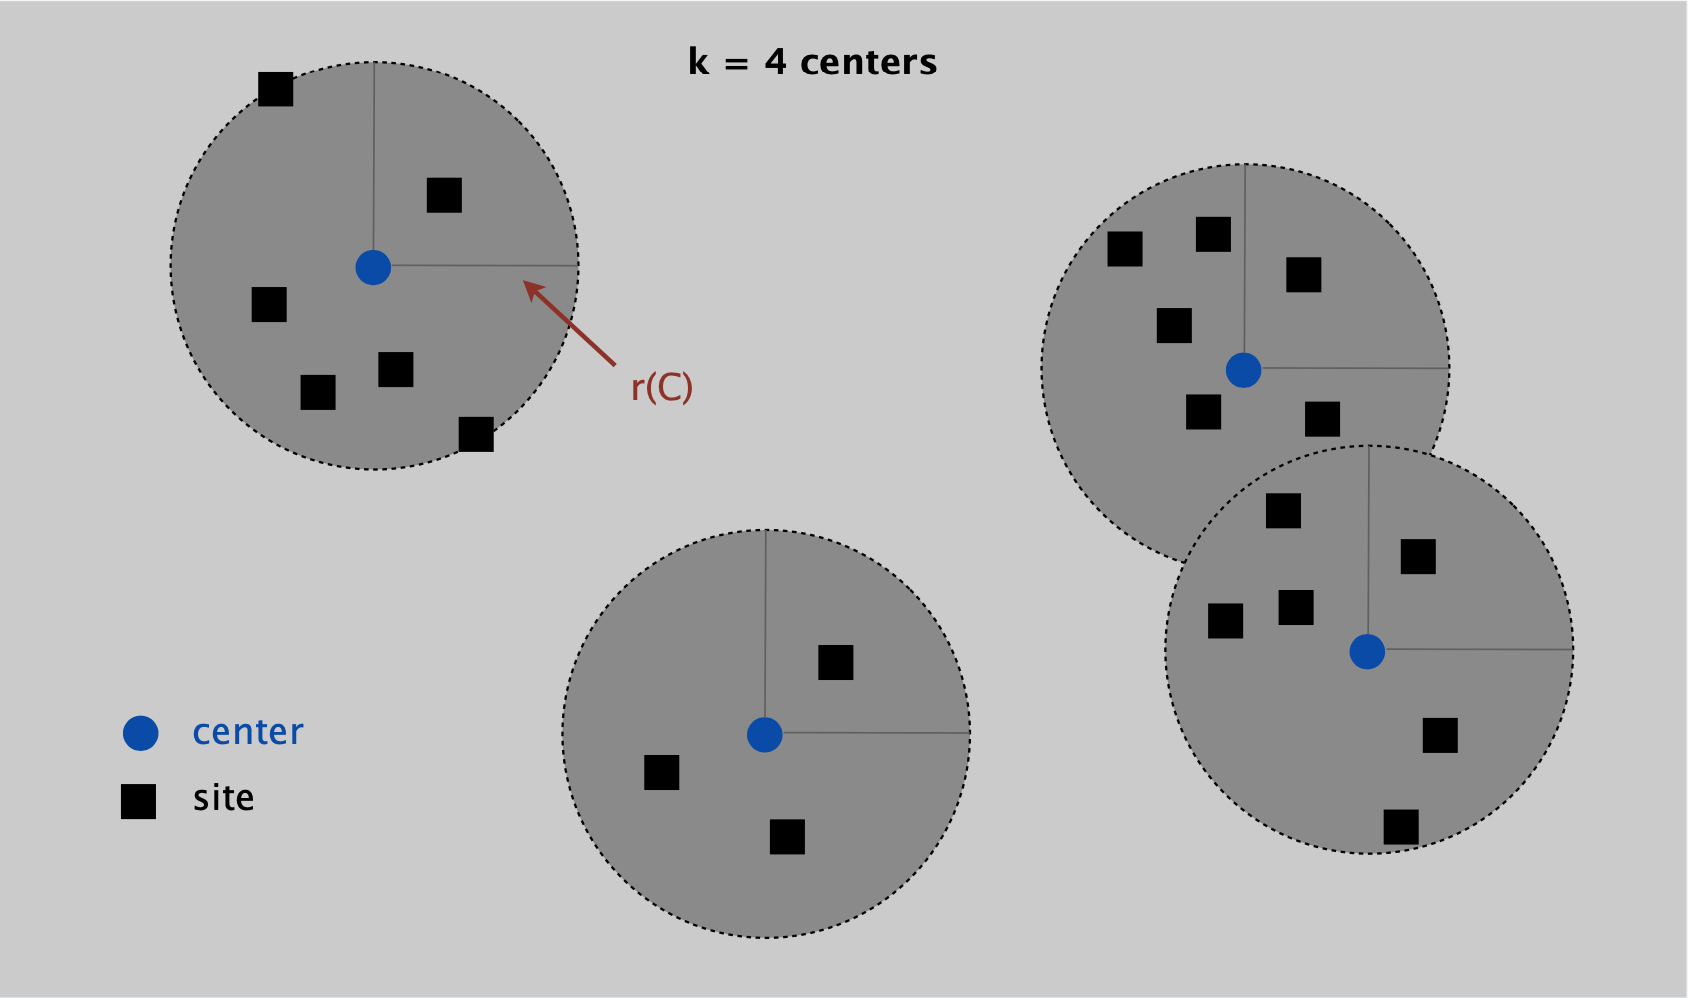
\includegraphics[width=0.6\textwidth ]{kCenter}
    \caption{The k-center selection problem}
\end{figure}

\emph{Greedy Solution}: Put the first center at the best possible location for a single center, and then keep adding centers so as to reduce the covering radius each time by as much as possible (this solution is very bad).\\

\begin{claim}
    Let $C^{*}$ be an optimal set of centers. Then r(C) $\leq$ 2r($C^{*}$)
\end{claim}

\begin{proof}
    \begin{itemize}
        \item{Assume $r(C^{*}) < 1/2 r(C)$}.
        \item{For each site $ci \in C$, consider ball of radius 1/2 r(C) around it. Exactly one $ci^{*}$ in each ball; let $c_{i}$ be the site paired with $ci^{*}$. Consider any site s and its closest center $ci^{*} ∈ C^{*}$}
        \item{$dist(s, C) \leq dist(s, ci) \leq dist(s, ci^{*}) + dist(ci_{*}, ci) \leq 2r(C^{*}).$}
        \item{Thus, $r(C) \leq 2r(C^{*})$}
    \end{itemize}
\end{proof}

\begin{figure}[H]
    \centering
    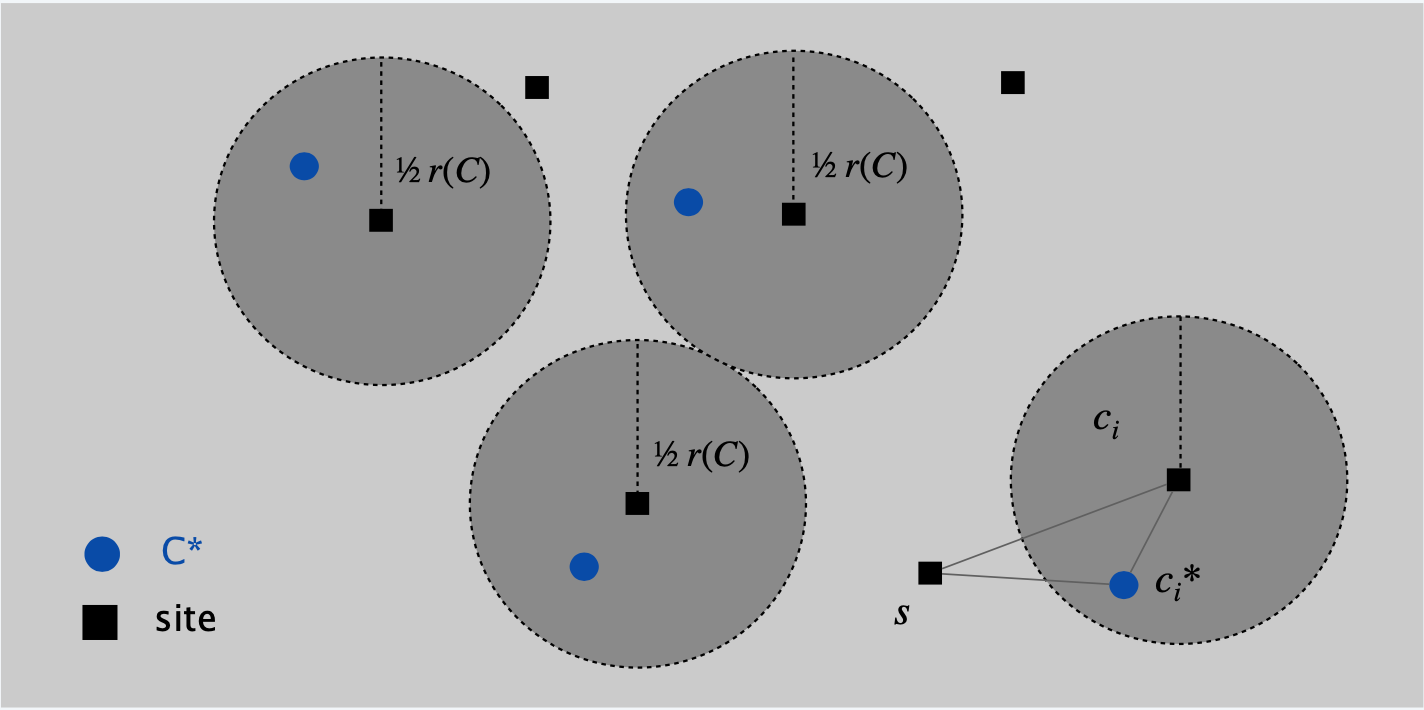
\includegraphics[width=0.6\textwidth ]{kCenterDemonstration}
\end{figure}

\begin{claim}
    Unless P = NP, there no ρ-approximation for center selection problem for any $ρ < 2$.
\end{claim}\\

\begin{proof}
    We show how we could use a (2 – ε) approximation algorithm for CENTER-SELECTION selection to solve DOMINATING-SET in poly-time:
    \begin{itemize}
        \item{Let G = (V, E), k be an instance of DOMINATING-SET (a dominating set for a graph G = (V, E) is a subset D of V such that every vertex not in D is adjacent to at least one member of D)}
        \item{Construct instance $G^{'}$ of CENTER-SELECTION with sites V and distances}
        \item{$dist(u, v) = 1 if (u, v) \in E$ $dist(u, v) = 2 if (u, v) \notin E$}
        \item{Note that $G^{'}$ satisfies the triangle inequality.}
        \item{G has dominating set of size k if there exists k centers C* with r(C*) = 1.}
    \end{itemize}

    Thus, if G has a dominating set of size k, a (2 – ε)approximation algorithm for CENTER-SELECTION would find a solution C* with r(C*) = 1 since it cannot use any edge of distance 2.
\end{proof}

\subsection{Knapsack Problem}
PTAS: (1 + ε)-approximation algorithm for any constant ε > 0, produces arbitrarily high quality solution, but trades off accuracy for time.\\\\
The knapsack problem is the same as seen 4.2, in general we get further from the desired value while respecting the weight limit W:\\\\
Given a set X, weights wi ≥ 0, values vi ≥ 0, a weight limit W, and a target value V, is there a subset S ⊆ X such that:

\[\begin{cases} \sum_{i \in S} w_{i} \leq W \\  \sum_{i \in S} v_{i} \geq V \end{cases}\]

\begin{claim}
    SUBSET-SUM $\leq _{p}$ KNAPSACK
\end{claim}

\begin{figure}[H]
    \centering
    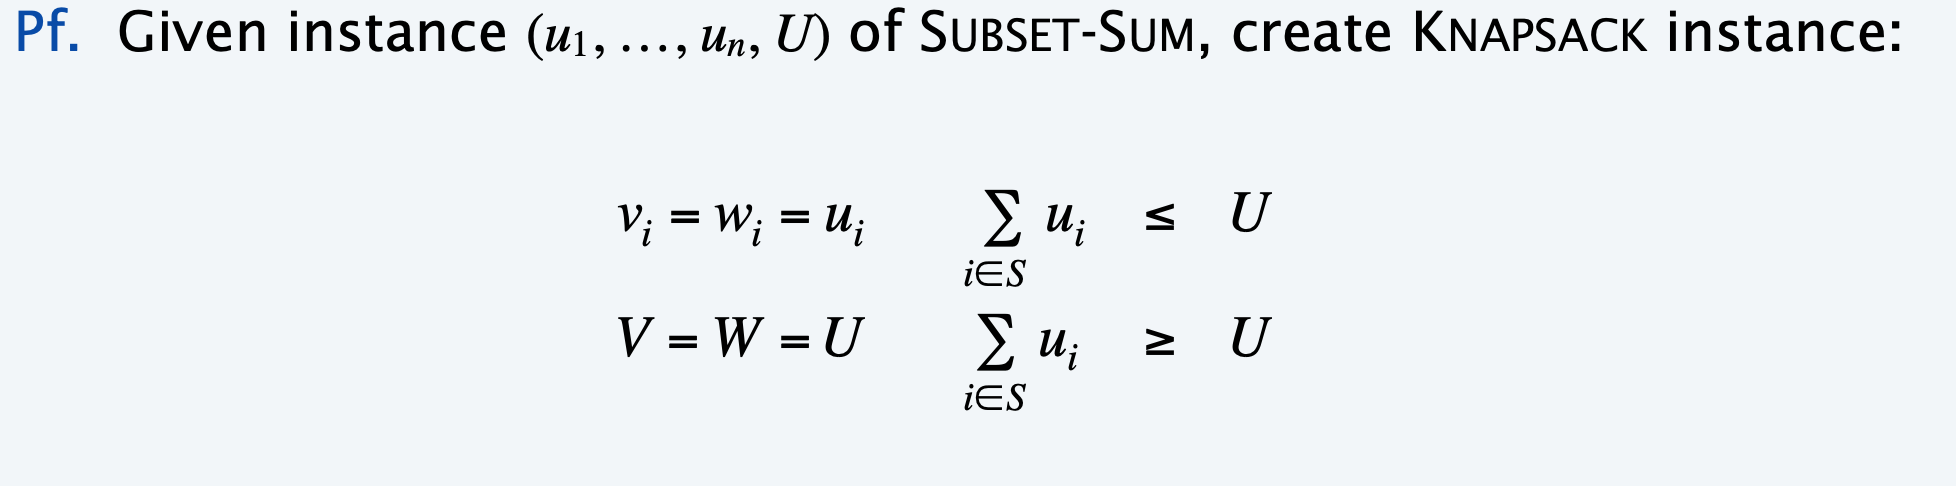
\includegraphics[width=0.6\textwidth ]{NPKnapsack}
    \caption{Knapsack problem reduction}
\end{figure}

\begin{figure}[H]
    \centering
    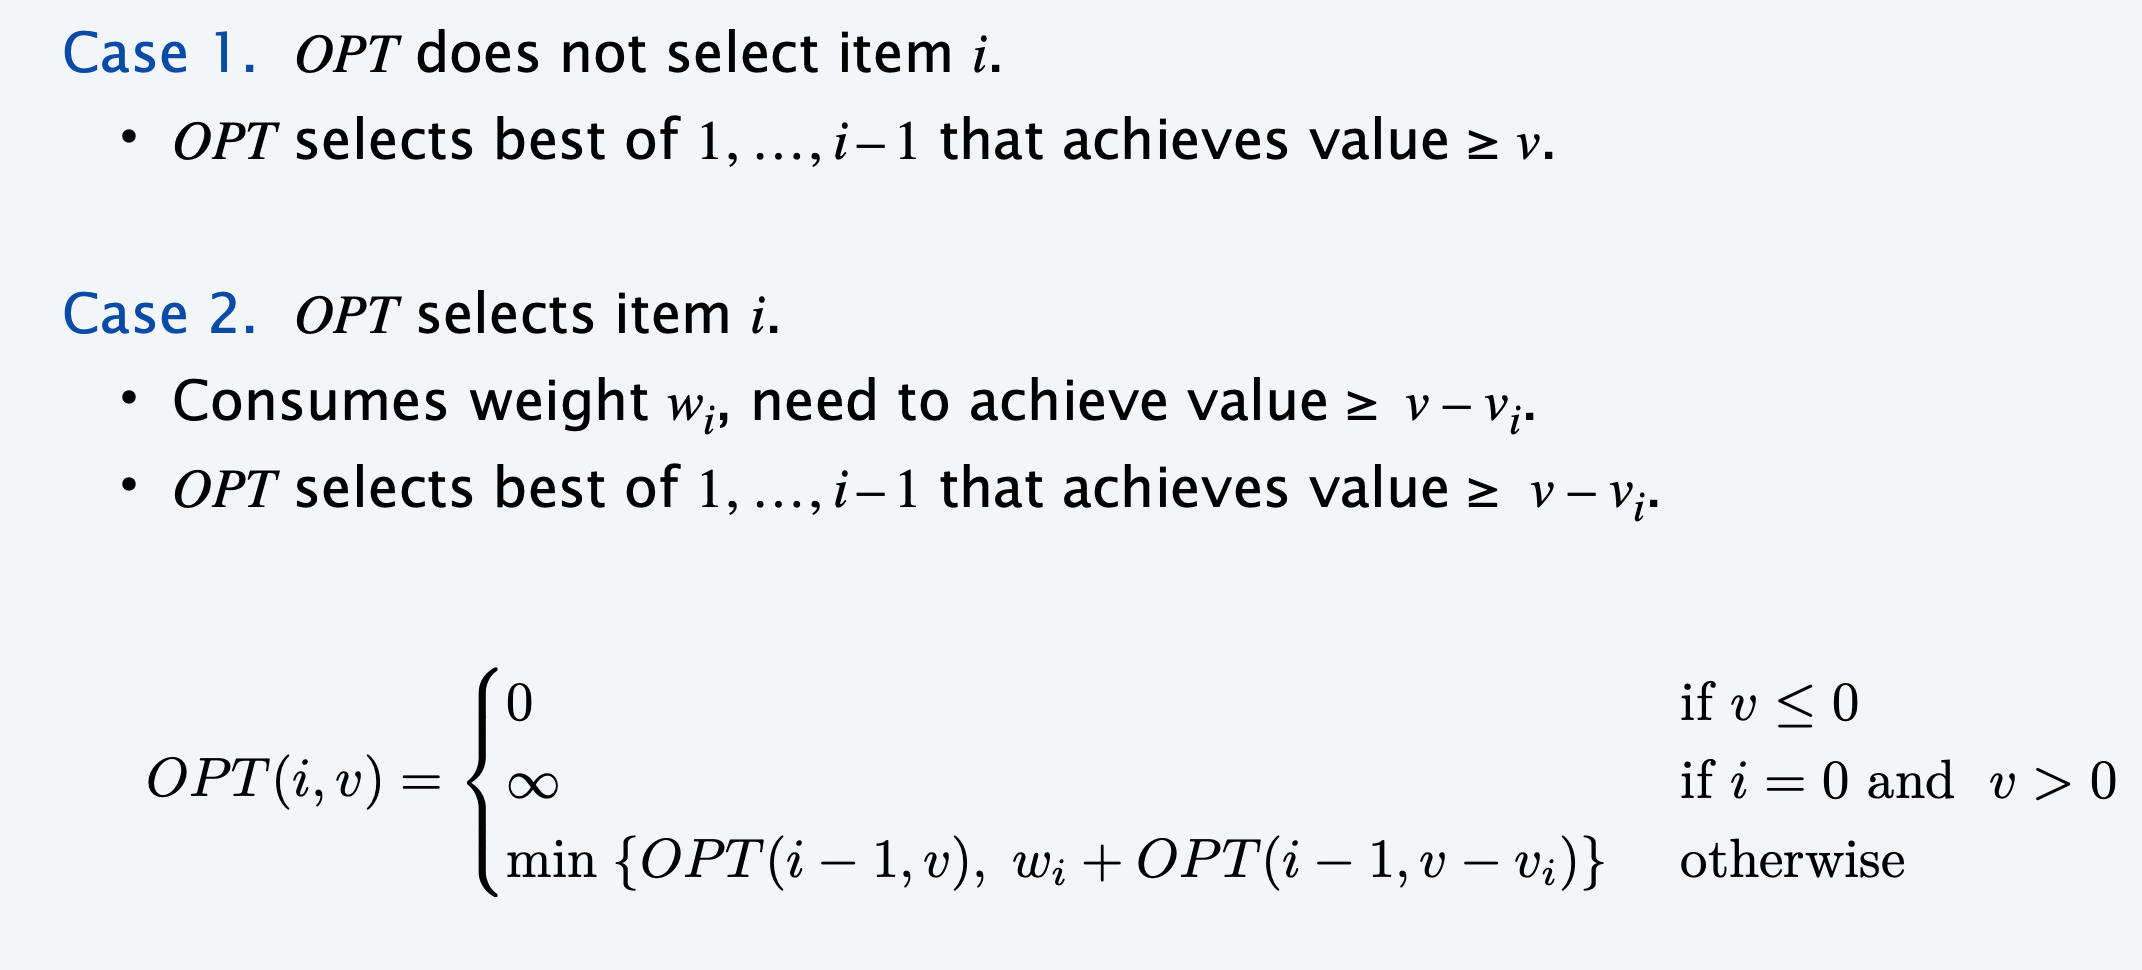
\includegraphics[width=0.6\textwidth ]{knapsackII}

\end{figure}
The approximation should do the following: round all values up to lie in smaller range, then run dynamic programming algorithm II on rounded/scaled instance.

\begin{itemize}
    \item{$0<ε\leq1$ it's the precision parameter}
    \item{$v_{max}$ is the largest value of the original instances}
    \item{$\theta$ = scaling factor }
\end{itemize}

Observation. Optimal solutions to problem with v are equivalent to the optimal solution v*.

For any ε $>$ 0, the rounding algorithm computes a feasible solution whose value is within a (1 + ε) factor of the optimum in O(n3 / ε) time.

\clearpage
